\documentclass[11pt]{article}
\newcommand{\doctitle}{RV32I CPU — Verification Specification}
\newcommand{\docsubject}{Reproducible stimuli, checks and waveform evidence}
\newcommand{\docrev}{2.1}
\newcommand{\docdate}{21 September 2026}
% ---------------------------------------------------------------------------
% Shared preamble for the specification set.
% Compiled with LuaLaTeX.
% ---------------------------------------------------------------------------
\usepackage{fontspec}
\setmainfont{Latin Modern Roman}[SmallCapsFont={Latin Modern Roman Caps}]
\setsansfont{Latin Modern Sans}
\setmonofont{Latin Modern Mono}[BoldFont={Latin Modern Mono}]

\usepackage[a4paper,top=27mm,bottom=25mm,left=25mm,right=22mm,headheight=15pt]{geometry}

\usepackage{amsmath}
\usepackage{amssymb}
\usepackage{booktabs}
\usepackage{longtable}
\usepackage{tabularx}
\usepackage{array}
\usepackage{multirow}
\usepackage{enumitem}
\usepackage{xcolor}
\usepackage{fancyhdr}
\usepackage{titlesec}
\usepackage{caption}
\usepackage{float}
\usepackage{graphicx}
\usepackage{tikz}
\usepackage{tikz-timing}
\usetikzlibrary{arrows.meta,positioning,automata,calc,fit,backgrounds,
                shapes.geometric,shapes.misc,decorations.pathreplacing}
\usepackage[hidelinks,bookmarksnumbered]{hyperref}

% --- palette ---------------------------------------------------------------
\definecolor{accent}{RGB}{0,72,110}
\definecolor{rulegrey}{RGB}{120,120,120}
\definecolor{boxbg}{RGB}{244,246,248}

% --- head / foot -----------------------------------------------------------
\pagestyle{fancy}
\fancyhf{}
\fancyhead[L]{\small\nouppercase{\leftmark}}
\fancyhead[R]{\small\thepage}
\fancyfoot[L]{\footnotesize\doctitle}
\fancyfoot[R]{\footnotesize Rev.\ \docrev\ --- \docdate}
\renewcommand{\headrulewidth}{0.4pt}
\renewcommand{\footrulewidth}{0.4pt}
\fancypagestyle{plain}{%
  \fancyhf{}%
  \fancyfoot[L]{\footnotesize\doctitle}%
  \fancyfoot[R]{\footnotesize Rev.\ \docrev\ --- \docdate}%
  \renewcommand{\headrulewidth}{0pt}%
  \renewcommand{\footrulewidth}{0.4pt}%
}

\titleformat{\section}{\normalfont\Large\bfseries\color{accent}}{\thesection}{0.7em}{}
\titleformat{\subsection}{\normalfont\large\bfseries}{\thesubsection}{0.7em}{}
\titleformat{\subsubsection}{\normalfont\normalsize\bfseries}{\thesubsubsection}{0.7em}{}
\titlespacing*{\section}{0pt}{16pt}{8pt}

\captionsetup{font=small,labelfont={bf,color=accent},skip=5pt}
\setcounter{secnumdepth}{3}
\setcounter{tocdepth}{3}

% --- macros ----------------------------------------------------------------
\newcommand{\sig}[1]{\texttt{#1}}
\newcommand{\reg}[1]{\texttt{#1}}

\newcolumntype{L}[1]{>{\raggedright\arraybackslash}p{#1}}
\newcolumntype{C}[1]{>{\centering\arraybackslash}p{#1}}

\tikzset{
  blk/.style={draw=accent,fill=white,rounded corners=1.5pt,align=center,
              inner sep=5pt,font=\small,minimum height=9mm},
  blkf/.style={blk,fill=boxbg},
  regbox/.style={draw=rulegrey,fill=boxbg,align=center,inner sep=4pt,font=\footnotesize},
  flow/.style={-{Stealth[length=2.4mm]},thick,draw=accent},
  flowd/.style={flow,dashed},
  lbl/.style={font=\scriptsize,inner sep=1.5pt,fill=white},
  stb/.style={draw=accent,fill=white,rounded corners=2pt,align=center,
              font=\small,inner xsep=5pt,inner ysep=4pt,
              minimum height=8mm,minimum width=19mm},
  stbi/.style={stb,double,double distance=0.6pt},
}

% identification block used on the title page of every document in the set
\providecommand{\docsubject}{}
\newcommand{\identblock}[1]{%
\begin{center}
\begin{tabular}{@{}L{0.28\linewidth}L{0.60\linewidth}@{}}
\toprule
Document & \doctitle \\
Document type & #1 \\
Subject & \docsubject \\
Revision & \docrev \\
Date & \docdate \\
Author & Bunea Cosmin-Andrei \\
Status & Released for review \\
\bottomrule
\end{tabular}
\end{center}}

\begin{document}
\begin{titlepage}\vspace*{24mm}
{\Huge\bfseries\color{accent}RV32I CPU\par}\vspace{4mm}{\LARGE Verification Specification\par}\vspace{12mm}
{\Large Reproducible stimuli, checks and waveform evidence\par}\vfill
\identblock{Verification specification}\end{titlepage}
\tableofcontents
\clearpage
\section{Introduction}

\needspace{7\baselineskip}
\subsection{Purpose of the document}
\noindent This specification describes the simulation strategy, stimulus, reference models and acceptance checks of the RV32I three-stage CPU. It is intended for hardware designers, verification engineers and software developers integrating the block.\par\medskip
\noindent It defines the behaviour that the RTL must show at its interfaces.\par\medskip

\needspace{7\baselineskip}
\subsection{Validity of the document}
\noindent The documented configuration is the RTL in cpu/hdl and the associated CPU/PIC and SoC simulation environments. Interface adaptations from the supplied briefs are identified in the integration section.\par\medskip
\noindent Revision 2.1 of 21 September 2026 describes the delivered state of that RTL.\par\medskip

\needspace{7\baselineskip}
\subsection{Terms and abbreviations}
{\small
\begin{longtable}{@{}L{0.2300\dimexpr\linewidth-12pt\relax}L{0.7700\dimexpr\linewidth-12pt\relax}@{}}
\toprule
\textbf{Term} & \textbf{Meaning} \\ \midrule
\endfirsthead
\toprule
\textbf{Term} & \textbf{Meaning} \\ \midrule
\endhead
AXI4-Lite & Single-beat AXI read/write channels. \\ \addlinespace[3pt]
BHT / BTB & Branch direction / target tables. \\ \addlinespace[3pt]
CSR & Control and status register. \\ \addlinespace[3pt]
DUT & Device under test. \\ \addlinespace[3pt]
EOI & End of interrupt; completes one service level. \\ \addlinespace[3pt]
IRQ & Interrupt request. \\ \addlinespace[3pt]
LSU & Load/store unit. \\ \addlinespace[3pt]
NBA & Nonblocking-assignment update region in simulation. \\ \addlinespace[3pt]
PIC & Programmable interrupt controller. \\ \addlinespace[3pt]
RAS & Return-address stack. \\ \addlinespace[3pt]
S1 / S2 / S3 & Fetch / decode-execute / writeback. \\ \addlinespace[3pt]
SVA & SystemVerilog Assertions. \\ \addlinespace[3pt]
\bottomrule\end{longtable}}

\clearpage
\subsection{Relationship with other documents}
\noindent The documents below are the ones this specification is derived from or read with.\par\medskip
{\small
\begin{longtable}{@{}L{0.5000\dimexpr\linewidth-12pt\relax}L{0.5000\dimexpr\linewidth-12pt\relax}@{}}
\toprule
\textbf{Reference} & \textbf{Version / role} \\ \midrule
\endfirsthead
\toprule
\textbf{Reference} & \textbf{Version / role} \\ \midrule
\endhead
RV32I 3-Stage Pipeline CPU.pdf & Supplied project draft; functional requirements and implementation decisions. \\ \addlinespace[3pt]
Spec table of contents and templates.pdf & Supplied document structure and verification-plan template. \\ \addlinespace[3pt]
Design Specification — CPU & Companion specification, revision 2.1, 21 September 2026. \\ \addlinespace[3pt]
RISC-V Unprivileged ISA / Privileged Architecture & v20191213 / v20211203, machine mode \\ \addlinespace[3pt]
ARM IHI0022E / IEEE 1364-2005 & AXI4-Lite / Verilog RTL. \\ \addlinespace[3pt]
\bottomrule\end{longtable}}

\needspace{7\baselineskip}
\subsection{Notes on the notation used}
\noindent Signal and register names follow the RTL. Addresses and waveform bus values are hexadecimal; time is in ns and widths are in bits. Register offsets are byte offsets; CSR addresses are instruction-encoded indices.\par\medskip
{\small
\begin{longtable}{@{}L{0.2600\dimexpr\linewidth-12pt\relax}L{0.7400\dimexpr\linewidth-12pt\relax}@{}}
\toprule
\textbf{Notation} & \textbf{Meaning} \\ \midrule
\endfirsthead
\toprule
\textbf{Notation} & \textbf{Meaning} \\ \midrule
\endhead
Fixed-width name & A Verilog module, port, file or script name, spelled as in the source. \\ \addlinespace[3pt]
Signal suffix \_i / \_o & Module input / output, seen from inside that module. \\ \addlinespace[3pt]
[a:b] & Bit range, most significant bit first. \\ \addlinespace[3pt]
S1 / S2 / S3 & Pipeline stage names used throughout the document. \\ \addlinespace[3pt]
posedge +1 ns & A testbench stimulus time, one nanosecond after the sampling edge. \\ \addlinespace[3pt]
\bottomrule\end{longtable}}

\clearpage
\section{Verification methodology}
\subsection{Overview and acceptance}
\noindent A run either passes or fails; this section states what that verdict covers. The first table gives the acceptance conditions applied to every test and the limits of what simulation shows; the second gives the runs behind the results quoted in this document.\par\medskip
{\small
\begin{longtable}{@{}L{0.2900\dimexpr\linewidth-12pt\relax}L{0.7100\dimexpr\linewidth-12pt\relax}@{}}
\toprule
\textbf{Item} & \textbf{Contract} \\ \midrule
\endfirsthead
\toprule
\textbf{Item} & \textbf{Contract} \\ \midrule
\endhead
Requirement source & RV32I 3-Stage Pipeline CPU.pdf \\ \addlinespace[3pt]
Device under test & rv32i\_cpu\_top and its RTL modules. \\ \addlinespace[3pt]
Functional verdict & Every expected value and response must match; errors=0 and test\_done=1 are required. \\ \addlinespace[3pt]
Protocol verdict & VALID/payload stability, response ordering and outstanding transaction limits; clocked at posedge. \\ \addlinespace[3pt]
Failure handling & Mismatch, timeout, incomplete test, assertion failure or coverage-gate failure returns a failing run. \\ \addlinespace[3pt]
Limits of evidence & Directed simulation and reference-model checks, not a formal proof or a synthesis/timing result. \\ \addlinespace[3pt]
\bottomrule\end{longtable}}
{\small
\begin{longtable}{@{}L{0.2900\dimexpr\linewidth-12pt\relax}L{0.7100\dimexpr\linewidth-12pt\relax}@{}}
\toprule
\textbf{Simulator / flow} & \textbf{Recorded evidence (18–21 September 2026)} \\ \midrule
\endfirsthead
\toprule
\textbf{Simulator / flow} & \textbf{Recorded evidence (18–21 September 2026)} \\ \midrule
\endhead
ModelSim & 22 CPU/PIC configurations; zero mismatches. \\ \addlinespace[3pt]
Verilator --assert & 16 CPU/PIC benches and the CPU functional-coverage gate. \\ \addlinespace[3pt]
Integrated SoC & 25 ModelSim configurations and 16 assertion-enabled benches. \\ \addlinespace[3pt]
PULP comparison & Decoder sequence plus 96 register-slave strobe/order/stall cases and RO/unmapped/reset cases. \\ \addlinespace[3pt]
\bottomrule\end{longtable}}

\clearpage
\subsection{Implementation strategy and reference model}
\noindent Directed tests exercise individual features and simultaneous events. Program/reference tests check end-to-end results. Protocol checks observe accepted transfers; state checks sample after nonblocking updates.\par\medskip
\noindent The ISA reference generates an instruction-by-instruction expected trace and memory state. The CPU runs the same sequence with nominal and delayed responders.\par\medskip
\noindent The verification plan records an ID, scenario, expected result, status and test/checker. Its detailed cases appear in the annex; the environment below identifies the components that execute and check them.\par\medskip

\clearpage
\section{Verification environment}
\subsection{Overview}

\noindent The program image supplies instructions and initial data to the responders. Checks compare observed architectural state with expected results, while protocol monitors and assertions inspect the bus and pipeline independently.\par
\begin{figure}[H]\centering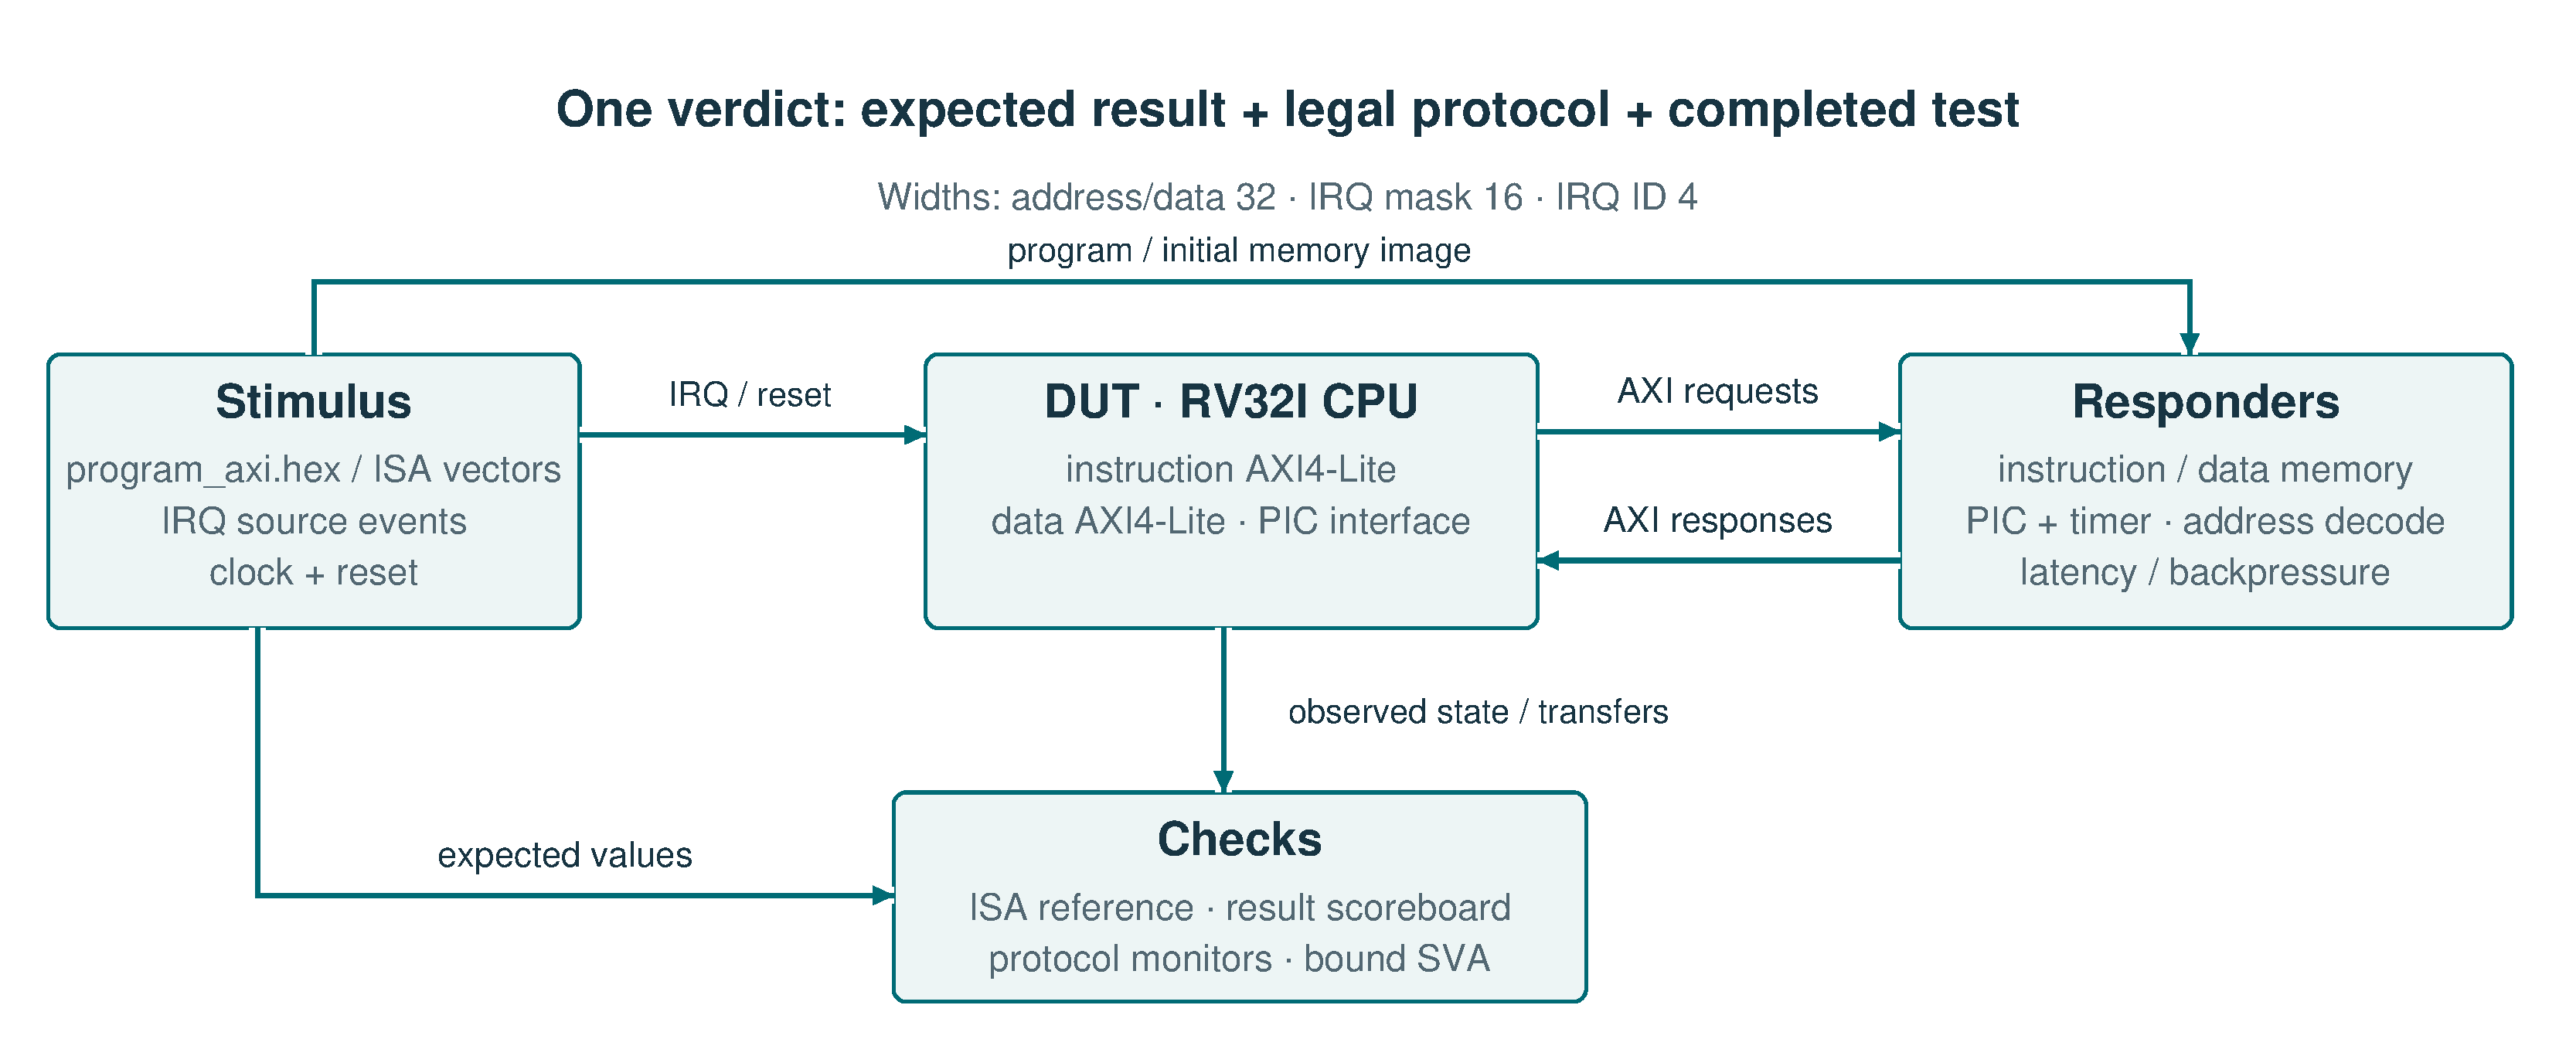
\includegraphics[width=\linewidth,height=105mm,keepaspectratio]{figures/cpu_verification.pdf}\caption{Test stimuli, DUT and independent checking paths.}\end{figure}
{\small
\begin{longtable}{@{}L{0.2400\dimexpr\linewidth-12pt\relax}L{0.7600\dimexpr\linewidth-12pt\relax}@{}}
\toprule
\textbf{Component} & \textbf{File / role} \\ \midrule
\endfirsthead
\toprule
\textbf{Component} & \textbf{File / role} \\ \midrule
\endhead
Clock / reset & ck\_rst\_tb.v: shared generator; dedicated reset benches can drive a reset pulse between edges. \\ \addlinespace[3pt]
Bus stimulus & tb\_axil\_master.vh: register-access tasks; CPU programs supply real load/store requests at system level. \\ \addlinespace[3pt]
Memory model & axi\_lite\_mem\_model.v: configurable response delay and repeatable backpressure. \\ \addlinespace[3pt]
Reference & isa\_reference.py: instruction trace. \\ \addlinespace[3pt]
Verdict & tb\_check.vh: explicit mismatch count, completion and fatal failure. \\ \addlinespace[3pt]
Protocol & axi\_lite\_monitor.v for ModelSim; axi\_lite\_sva.sv under Verilator. \\ \addlinespace[3pt]
\bottomrule\end{longtable}}

\clearpage
\subsection{Control and drivers}
\noindent Stimulus is driven one nanosecond after the sampling edge, so that a test never races the design it is checking. The table gives the timing rule for each driven event and the reason for it; the waveform shows the reset case, the one event placed off the clock grid.\par\medskip
{\small
\begin{longtable}{@{}L{0.2400\dimexpr\linewidth-24pt\relax}L{0.4200\dimexpr\linewidth-24pt\relax}L{0.3400\dimexpr\linewidth-24pt\relax}@{}}
\toprule
\textbf{Signal / event} & \textbf{Timing rule} & \textbf{Reason} \\ \midrule
\endfirsthead
\toprule
\textbf{Signal / event} & \textbf{Timing rule} & \textbf{Reason} \\ \midrule
\endhead
clk & 10 ns period in these traces; rising edges are 5, 15, 25… ns. & Defines the handshake observation points. \\ \addlinespace[3pt]
Shared bus / claim tasks & Drive 1 ns after posedge, in a separate statement. Hold until the sampling edge. & Avoid blocking-assignment races with DUT active/NBA evaluation. \\ \addlinespace[3pt]
Handshake observation & Sample VALID \&\& READY at posedge before changing stimulus. & Records the transfer that the DUT accepted. \\ \addlinespace[3pt]
Reset assertion & Dedicated reset tests assert at posedge +2 ns, check at +3 ns. & The check occurs before either the next falling or rising edge. \\ \addlinespace[3pt]
Reset release & Explicit nanosecond delays, off the clock grid; shared generator releases at 123 ns. & Exercises asynchronous stimulus without a coincident clock event. \\ \addlinespace[3pt]
\bottomrule\end{longtable}}

\noindent Reset is asserted while an instruction request is waiting. ARVALID clears at the reset event, before the next rising edge; after release the fetch request resumes from RESET\_PC.\par
\begin{figure}[H]\centering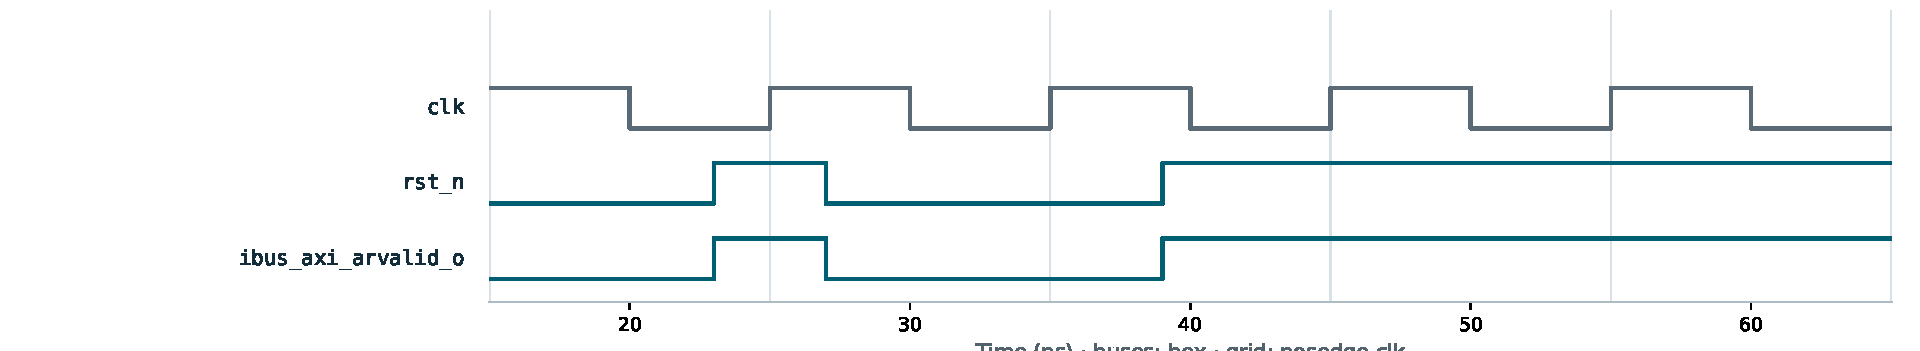
\includegraphics[width=\linewidth]{waves/cpu_reset.pdf}\caption{Reset from active state at posedge +2 ns; cleared state is checked at +3 ns.}\end{figure}
{\small
\begin{longtable}{@{}L{0.3000\dimexpr\linewidth-12pt\relax}L{0.7000\dimexpr\linewidth-12pt\relax}@{}}
\toprule
\textbf{Formatting convention} & \textbf{Code} \\ \midrule
\endfirsthead
\toprule
\textbf{Formatting convention} & \textbf{Code} \\ \midrule
\endhead
Separate statements & @(posedge clk); followed on the next line by \#1; and then the signal assignments. \\ \addlinespace[3pt]
Scope of \#1 & Applies to testbench scheduling only. \\ \addlinespace[3pt]
\bottomrule\end{longtable}}

\clearpage
\subsection{Monitors and checkers}
\noindent Checking is split between bus protocol and functional result, so that a failure points at one of the two. The first table lists each checker and what it observes; the second shows how each one is kept from passing without having seen traffic.\par\medskip
{\small
\begin{longtable}{@{}L{0.3600\dimexpr\linewidth-12pt\relax}L{0.6400\dimexpr\linewidth-12pt\relax}@{}}
\toprule
\textbf{File / mechanism} & \textbf{What it checks} \\ \midrule
\endfirsthead
\toprule
\textbf{File / mechanism} & \textbf{What it checks} \\ \midrule
\endhead
axi\_lite\_monitor.v & Passive ModelSim protocol checks and transaction counts; valid traffic must occur. \\ \addlinespace[3pt]
axi\_lite\_sva.sv & Channel stability, legal response codes, request/response ordering, one outstanding transaction per direction. \\ \addlinespace[3pt]
rv32i\_cpu\_core\_sva.sv & Pipeline/trap/forwarding invariants. \\ \addlinespace[3pt]
rv32i\_bind\_core\_sva.sv & bind attaches checker instances to RTL module types. The checkers read DUT signals; they drive nothing and add no port. \\ \addlinespace[3pt]
rv32i\_bind\_sva.sv & Attaches the nominal CPU functional-coverage model; coverage is separate from the shared assertion bind. \\ \addlinespace[3pt]
run\_verilator.sh & Compiles assertions with --assert and fails the run on an assertion failure. ModelSim ASE runs the procedural monitors instead; the SVA execute under Verilator. \\ \addlinespace[3pt]
\bottomrule\end{longtable}}
{\small
\begin{longtable}{@{}L{0.3200\dimexpr\linewidth-12pt\relax}L{0.6800\dimexpr\linewidth-12pt\relax}@{}}
\toprule
\textbf{Non-vacuous check} & \textbf{Evidence} \\ \midrule
\endfirsthead
\toprule
\textbf{Non-vacuous check} & \textbf{Evidence} \\ \midrule
\endhead
Valid traffic & Read/write counts and exercised tests prevent a disconnected monitor from being counted as coverage. \\ \addlinespace[3pt]
Preconditions & RO-write test first creates nonzero state; async-reset test first creates pending/nonzero state. \\ \addlinespace[3pt]
Negative scenarios & Watch an interval for forbidden offers/claims; do not infer absence from one sample. \\ \addlinespace[3pt]
\bottomrule\end{longtable}}

\clearpage
\subsection{Simulation environment setup}
\noindent The environment is a fixed folder layout plus a small number of named scripts. The tables give that layout, the exact command for each step in the order it is run, and the tools each step needs.\par\medskip
\needspace{7\baselineskip}\subsubsection{Structure}
{\small
\begin{longtable}{@{}L{0.2200\dimexpr\linewidth-12pt\relax}L{0.7800\dimexpr\linewidth-12pt\relax}@{}}
\toprule
\textbf{Folder} & \textbf{Contents} \\ \midrule
\endfirsthead
\toprule
\textbf{Folder} & \textbf{Contents} \\ \midrule
\endhead
cpu/hdl & Synthesizable RTL: the CPU modules, the PIC, the timer and the AXI4-Lite register front-end. \\ \addlinespace[3pt]
cpu/debug/hdl & Testbenches, bus masters and the configurable memory and responder models. \\ \addlinespace[3pt]
cpu/debug/sva & Assertion modules and the bind files that attach them to RTL module types. \\ \addlinespace[3pt]
cpu/debug/sim & Run scripts, file lists, reference models, generated programs and run logs. \\ \addlinespace[3pt]
soc/hdl & Integration fabric: address decode, arbitration, AXI4-Full to Lite conversion and RAM. \\ \addlinespace[3pt]
soc/debug/hdl, sva, sim & The same split as above, applied to the integrated SoC. \\ \addlinespace[3pt]
cpu/docs & Specification sources, generated figures and the waveform windows. \\ \addlinespace[3pt]
\bottomrule\end{longtable}}
\needspace{7\baselineskip}\subsubsection{Scripts}
{\small
\begin{longtable}{@{}L{0.0600\dimexpr\linewidth-36pt\relax}L{0.2200\dimexpr\linewidth-36pt\relax}L{0.4300\dimexpr\linewidth-36pt\relax}L{0.2900\dimexpr\linewidth-36pt\relax}@{}}
\toprule
\textbf{Step} & \textbf{Working directory} & \textbf{Command / script} & \textbf{Result} \\ \midrule
\endfirsthead
\toprule
\textbf{Step} & \textbf{Working directory} & \textbf{Command / script} & \textbf{Result} \\ \midrule
\endhead
1 & Repository root & make asm & Regenerate programs and independent reference vectors. \\ \addlinespace[3pt]
2 & cpu/debug/sim & vsim -c -do "do regress.do; quit -f" & Compile and run 22 CPU/PIC configurations. \\ \addlinespace[3pt]
3 & cpu/debug/sim (Bash / WSL) & bash run\_verilator.sh & Lint, functional coverage and 16 benches with SVA. \\ \addlinespace[3pt]
4 & soc/debug/sim & vsim -c -do "do regress.do; quit -f" & 25 integration configurations. \\ \addlinespace[3pt]
5 & Repository root (Bash / WSL) & bash soc/debug/sim/run\_verilator.sh & SoC lint and 16 assertion-enabled benches. \\ \addlinespace[3pt]
6 & soc/debug/sim (Bash / WSL) & bash run\_pulp\_compare.sh & Pinned external decoder/register comparison. \\ \addlinespace[3pt]
7 & cpu/debug/sim & vsim -c -do "do waves.do" & Run 8 checked benches and export VCD traces. \\ \addlinespace[3pt]
8 & Repository root & python cpu/docs/tools/waveforms.py & SVG/PDF/PNG figures and source-window manifest. \\ \addlinespace[3pt]
\bottomrule\end{longtable}}
\needspace{7\baselineskip}\subsubsection{Setup and configuration}
{\small
\begin{longtable}{@{}L{0.2600\dimexpr\linewidth-12pt\relax}L{0.7400\dimexpr\linewidth-12pt\relax}@{}}
\toprule
\textbf{Tool / setup} & \textbf{Requirement} \\ \midrule
\endfirsthead
\toprule
\textbf{Tool / setup} & \textbf{Requirement} \\ \midrule
\endhead
ModelSim & vsim/vlog on PATH; run from the named simulation directory so file lists resolve. \\ \addlinespace[3pt]
Verilator & Verilator 5.050 used for the recorded run; C++ build tools, Bash and Python 3 are required. \\ \addlinespace[3pt]
PULP & Git and network only for the initial checkout; explicit revision pins recorded in the runner. \\ \addlinespace[3pt]
Wave rendering & Python with matplotlib; raw VCD files produced by waves.do. \\ \addlinespace[3pt]
Configuration & Latency/stall overrides are read back after elaboration; seeds are fixed for repeatability. \\ \addlinespace[3pt]
\bottomrule\end{longtable}}

\clearpage
\section{Annex}
\subsection{Verification plan}
\noindent PASS indicates the recorded regression completed with its expected results and zero checker errors. Each row identifies the test that exercises the listed behavior.\par\medskip
{\small
\begin{longtable}{@{}L{0.0800\dimexpr\linewidth-48pt\relax}L{0.1600\dimexpr\linewidth-48pt\relax}L{0.3700\dimexpr\linewidth-48pt\relax}L{0.1000\dimexpr\linewidth-48pt\relax}L{0.2900\dimexpr\linewidth-48pt\relax}@{}}
\toprule
\textbf{ID} & \textbf{Title} & \textbf{Expected result / scope} & \textbf{Status} & \textbf{Test / checker} \\ \midrule
\endfirsthead
\toprule
\textbf{ID} & \textbf{Title} & \textbf{Expected result / scope} & \textbf{Status} & \textbf{Test / checker} \\ \midrule
\endhead
CPU-01 & CPU integration & Arithmetic, logic, load/store, trap/IRQ/WFI programs; memory/register results and protocol monitors. & PASS & rv32i\_tb\_cpu\_axi \\ \addlinespace[3pt]
CPU-02 & ISA reference & 1287-instruction independently generated reference trace; nominal, delayed and stalled memories. & PASS & rv32i\_tb\_isa \\ \addlinespace[3pt]
CPU-03 & ALU & ALU operations, signed/unsigned boundaries and shifts. & PASS & rv32i\_tb\_alu \\ \addlinespace[3pt]
CPU-04 & Predictor / RAS & Tagged lookup, direction update, collisions, RAS push/pop/overflow/disabled setting and reset. & PASS & rv32i\_tb\_bp \\ \addlinespace[3pt]
CPU-05 & Exceptions / traps & All implemented synchronous causes; precedence, wrong-path errors and precise architectural state. & PASS & rv32i\_tb\_traps \\ \addlinespace[3pt]
CPU-06 & CSR access & CSR legality, fixed fields, write suppression, reserved modes and reset values. & PASS & rv32i\_tb\_csr\_ro \\ \addlinespace[3pt]
CPU-07 & Counters & Explicit write versus increment; half preservation, carry, CSRRS/CSRRC and fixed event IDs. & PASS & rv32i\_tb\_counters \\ \addlinespace[3pt]
CPU-08 & Two harts & Two distinct HART\_IDs on shared memory arbitration; no result corruption. & PASS & rv32i\_tb\_dual\_core \\ \addlinespace[3pt]
CPU-09 & Asynchronous reset & Reset between edges during fetch/load stall, nonzero GPR state, clock stopped, and resumed execution. & PASS & rv32i\_tb\_reset \\ \addlinespace[3pt]
\bottomrule\end{longtable}}

\clearpage
\subsection{Critical sequences}

\noindent The load holds S2 while its request or response is pending. At the RVALID/RREADY handshake, the data is available and s2\_advance permits the instruction to enter writeback.\par
\begin{figure}[H]\centering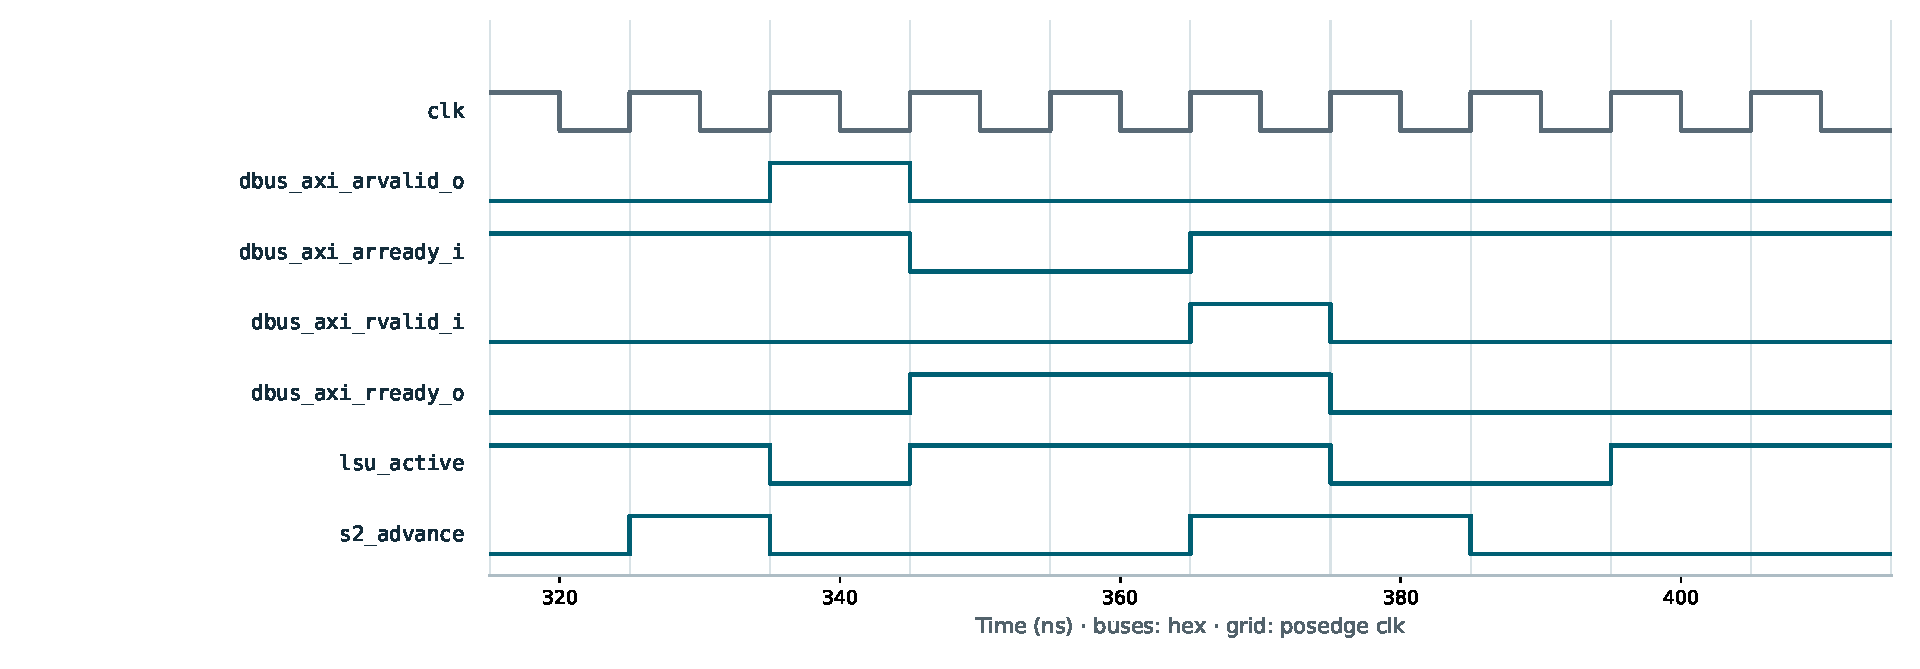
\includegraphics[width=\linewidth]{waves/cpu_load.pdf}\caption{Load completion and pipeline advance.}\end{figure}

\noindent The resolved branch differs from the prediction, causing redirect. IF/DX is invalidated so younger work cannot commit; an outstanding fetch response still completes its AXI transaction.\par
\begin{figure}[H]\centering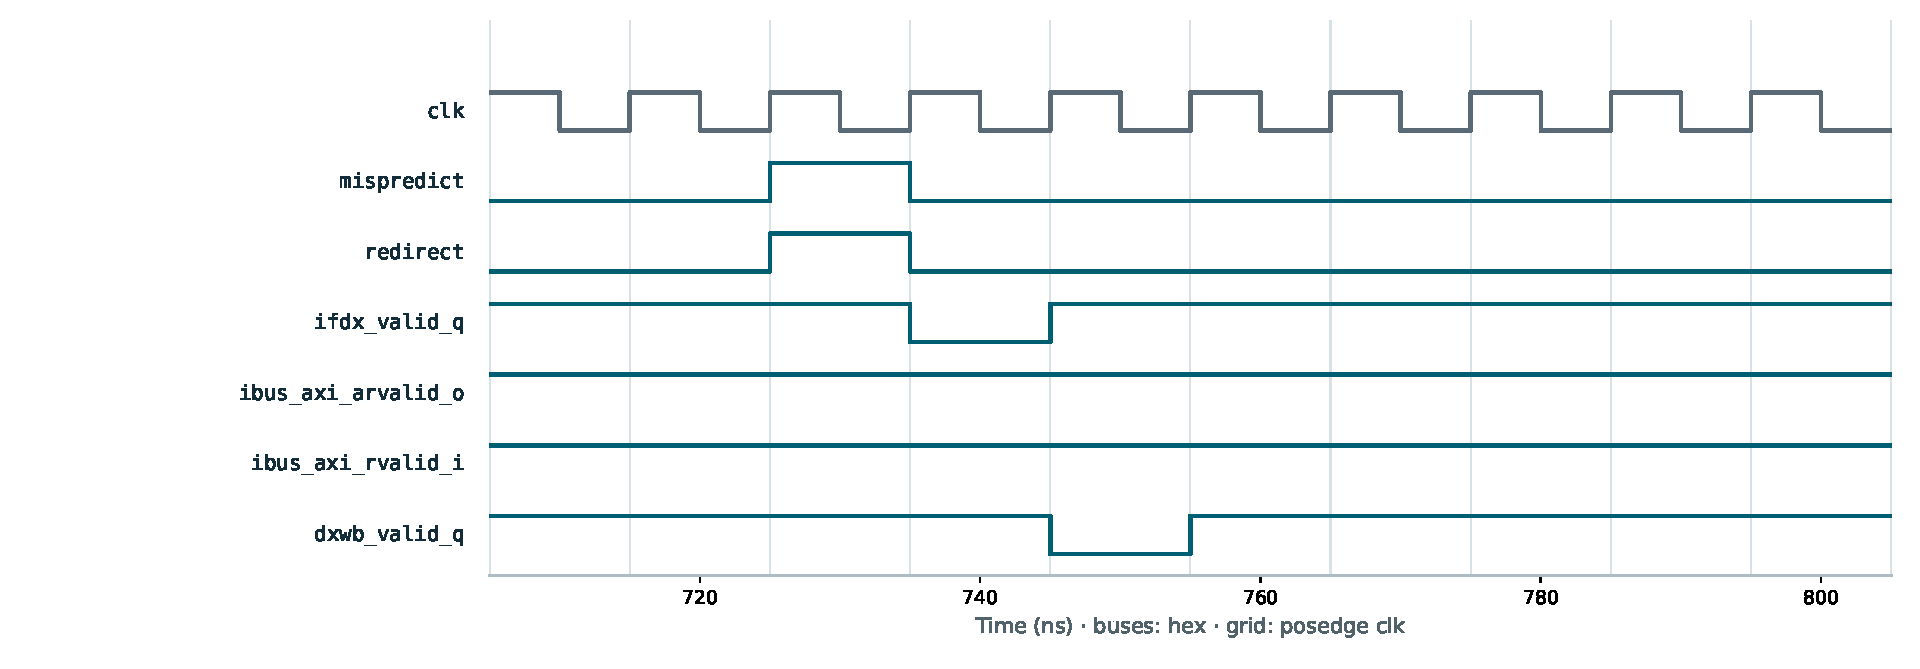
\includegraphics[width=\linewidth]{waves/cpu_redirect.pdf}\caption{Branch correction after a mispredicted branch.}\end{figure}
{\small
\begin{longtable}{@{}L{0.3000\dimexpr\linewidth-12pt\relax}L{0.7000\dimexpr\linewidth-12pt\relax}@{}}
\toprule
\textbf{Scenario} & \textbf{Check} \\ \midrule
\endfirsthead
\toprule
\textbf{Scenario} & \textbf{Check} \\ \midrule
\endhead
IRQ during load & No accepted IRQ until active LSU transaction is complete. \\ \addlinespace[3pt]
Wrong-path response error & Response is drained; wrong-path instruction cannot write GPR/CSR or trap. \\ \addlinespace[3pt]
Store channel skew & AW and W can complete in either order; one B response completes the store. \\ \addlinespace[3pt]
\bottomrule\end{longtable}}

\clearpage
\subsection{External AXI reference}
\noindent The AXI4-Lite front-end is compared against a published implementation to check the interpretation of the protocol. The first table states what was compared and on what evidence; the second names every difference found and what it means.\par\medskip
{\small
\begin{longtable}{@{}L{0.3200\dimexpr\linewidth-24pt\relax}L{0.3500\dimexpr\linewidth-24pt\relax}L{0.3300\dimexpr\linewidth-24pt\relax}@{}}
\toprule
\textbf{Compared block} & \textbf{Shared contract} & \textbf{Evidence} \\ \midrule
\endfirsthead
\toprule
\textbf{Compared block} & \textbf{Shared contract} & \textbf{Evidence} \\ \midrule
\endhead
soc\_axi\_lite\_dec vs axi\_lite\_demux & Two mapped targets, MaxTrans=1; independent progress and response timing. & Compare ordered data/response records and per-target address counts. \\ \addlinespace[3pt]
axi\_lite\_slave vs axi\_lite\_regs & 32-bit words; four RW words and one RO word; same byte strobes. & 96 cases = 16 WSTRB masks × 3 AW/W orders × 2 response-stall settings. \\ \addlinespace[3pt]
Additional register cases & RO write, unmapped access, reset and post-reset access. & Same access-class response and no forbidden state update; each side checked against expected data. \\ \addlinespace[3pt]
\bottomrule\end{longtable}}
{\small
\begin{longtable}{@{}L{0.2500\dimexpr\linewidth-12pt\relax}L{0.7500\dimexpr\linewidth-12pt\relax}@{}}
\toprule
\textbf{Difference / boundary} & \textbf{Interpretation} \\ \midrule
\endfirsthead
\toprule
\textbf{Difference / boundary} & \textbf{Interpretation} \\ \midrule
\endhead
Latency & Not cycle-identical; compare completed transactions and protocol compliance. \\ \addlinespace[3pt]
Unmapped read data & Our front-end returns zero; pinned PULP axi\_lite\_regs returns 0xBA5E1E55. Both return SLVERR; error-data policy is documented separately. \\ \addlinespace[3pt]
Address aliases & Different register-bank sizing; equality claimed only for the explicit compared address profile. \\ \addlinespace[3pt]
AXI4-Full & The PULP run does not establish equivalence of the DMA or soc\_axi\_full2lite to every upstream AXI4 module. \\ \addlinespace[3pt]
Converter & Local soc\_tb\_full2lite and soc\_tb\_full2lite\_err check supported burst handling and errors. Local write error aggregation preserves DECERR over SLVERR; PULP is not a cycle-exact reference for that policy. \\ \addlinespace[3pt]
Versions & axi: 70b8e54fd460e3308e58be596ceb3566a6e3576e; common\_cells: 03d98106aa19952a10360d2230def85144a0008b. \\ \addlinespace[3pt]
\bottomrule\end{longtable}}
\noindent Reference: \url{https://github.com/pulp-platform/axi}.

\end{document}
